\documentclass[a4paper,12pt,twoside]{article}
\usepackage[T1]{fontenc}
\usepackage[utf8]{inputenc}
\usepackage{lmodern}
\usepackage{url,csquotes}
\usepackage[hidelinks,hyperfootnotes=false]{hyperref}
\usepackage[titlepage,pagenumber]{polytechnique}
\usepackage{float}

\subtitle{MAP-536 - Python for Data Science}
\title{Final Project - Air data prediction}
\author{Leonardo \textsc{Natale} \& Guillaume \textsc{Le Fur}}
\logo{scikit_learn.jpeg}

\begin{document}

\maketitle

\section{Introduction}

The objective of this project was to predict a quantity related to the number of passengers on a given flight, on a given date. The data we were provided with initially was the following :

\begin{table}[H]
	\centering
	\begin{tabular}{|l|l|}
	\hline
	\textbf{Feature} & \textbf{Description}                          \\ \hline
	DateOfDeparture  & Date of departure                             \\ \hline
	Departure/Arrival& Departure and arrival airport                 \\ \hline
	WeeksToDeparture & Average number of weeks before departure when the ticket is booked \\ \hline
	log\_PAX          & Variable related to the number of passengers \\ \hline
	std\_wtd          & Standard deviation of WeeksToDeparture       \\ \hline
	\end{tabular}
	\label{table:orig_data}
\end{table}

The main goals were to become familiar with the way a machine learning project works, to apply the machine learning models we have seen in class and to become more proficient in Python.

\section{External Data and Data Preprocessing}

\subsection{External Data}

We have added the following data:

\begin{table}[H]
	\centering
	\begin{tabular}{|l|l|}
	\hline
	\textbf{Feature} & \textbf{Description}                        \\ \hline
	jet\_fuel        & Daily jet fuel price                        \\ \hline
	coordinates      & Airport geographical coordinates            \\ \hline
	gdp              & Departure and Arrival GDP                   \\ \hline
	passengers       & Monthly flow of passengers between airports \\ \hline
	holiday          & holiday data is the U.S.                    \\ \hline
	\end{tabular}
	\label{table:additional}
\end{table}

\subsection{Feature Engineering}



We were able to add the following extra features, by using the data described above:

\begin{table}[H]
	\centering
	\begin{tabular}{|l|l|}
	\hline
	\textbf{Feature} & \textbf{Description}                        \\ \hline
	closest holiday  & Number of days to the closest holiday.\\ \hline
	distance      	 & Distance in kilometers between departure and arrival airport.\\ \hline
	monthly\_logPAX   & Monthly log\_PAX per airport, both arrival and departure.  \\ \hline
	weekday\_logPAX   & log\_PAX per airport for every weekday.                    \\ \hline
	avg\_wtd          & Monthly average on WeeksToDeparture per airport.           \\ \hline
	avd\_std\_wtd      & Monthly average of std\_wtd per airport.                   \\ \hline
	\end{tabular}
	\label{table:feature_engineering}
\end{table}

\section{Infrastructure}

In order to test, optimize and integrate our models into the ramp infrastructure, we have come up with our own infrastructure, that enabled us to ease the testing and integration of new models. The structure is the following.

\begin{figure}[H]
	\centering
	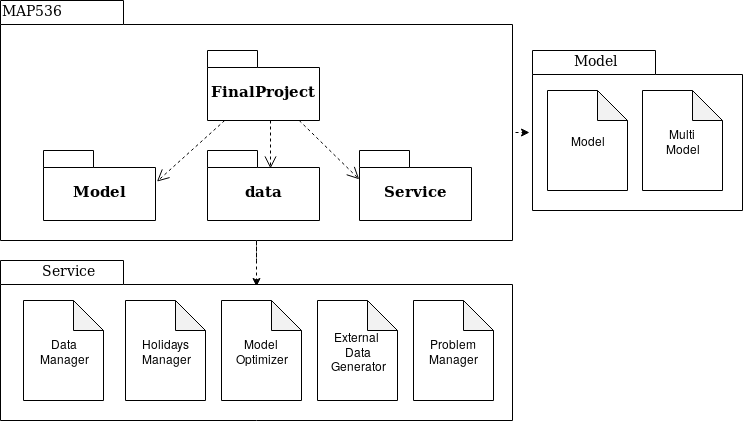
\includegraphics[scale=0.5]{UML.png}
\end{figure}

The \textbf{Data} folder contains all the external data files that we use to create our additional features. The \textbf{DataManager} is some kind of an interface between the model and the external data. It takes data as an input (either the train or test data) and merges it with external data, making it ready for fitting. It uses the \textbf{ExternalDataGenerator} which groups all our external data into the \textit{external\_data.csv} file. It is the class that is responsible for all the feature engineering of our models.\\
\textbf{Model} is a utility class that stores a sklearn model and two lists : a list of parameters that are to optimize via GridSearchCV and another with parameters that are to be optimized via RandomSearchCV. When used on RAMP, it's role is to contain the model and to fit and predict based on the data passed as an input. \textbf{MultiModel} is a class that goal is to simplify the testing of multiple models at the same time. \textbf{ModelOptimizer} is an interface, called by Model, that takes care of the RandomSearchCV and GridSearchCV and returns the result to Model.\\
\textbf{HolidaysManager} is a utility class used to vectorize operations on dates to determine whether they are holidays or how close they are to a holiday. \textbf{ProblemManager} is a class that contains metadata about the problem we intend to solve (columns that are relevant, external data we use, etc.)

\section{Models and Tuning}
\subsection{Models}

This table summarizes the train RMSE\footnote{The train and test RMSE values presented here are the one obtained locally as we couldn't submit the best models before the deadline of the project. Note that the score is often better on the RAMP server.} 

\begin{center}
	\begin{tabular}{| c | c | c | c |} 
		\hline
			 & Train RMSE & Test RMSE & Train time (s) \\ [0.5ex] 
		\hline
		\textbf{RandomForest} & 0.62 & 0.81 & 5.6 \\ 
		\hline
		\textbf{GradientBoostingRegressor} & 0.40 & 0.52 & 7.67 \\
		\hline
		\textbf{HistGradientBoostingRegressor} & 0.27 & 0.37 & 5.18 \\
		\hline
		\textbf{HistGradientBoostingRegressor (Tuned)} & \textbf{0.11} & \textbf{0.35} & \textbf{11.8} \\
		\hline
		\textbf{AdaBoostRegressor} & 0.19 & 0.34 & 107 \\
		\hline
	\end{tabular}
\end{center}


The Model we chose in the end is the \textbf{tuned HistGradientBoostingRegressor}, mostly because it's a good compromise between accuracy and training time. It's also the model that gives the best results without overfitting too much. Indeed, after a certain point ($RMSE_{test} \approx 0.35$), making the RMSE better by tuning hyper-parameters resulted in a very low training error ($RMSE_{train} < 0.10$), which we did not consider as acceptable.
Furthermore, the training time remains pretty low ($\approx 10 s$), which makes our model scalable. Indeed, even though we could achieve better performances with models that were longer to train, we though that an acceptable training time for a model fitted on 10000 rows would be around 10 seconds.

\subsection{Hyper-parameter Tuning vs Feature Importance}

During the project, we tried several models, made some hyper-parameter tuning and also added features along the way. We thought it would be interesting to keep track of the evolution of the value of our RMSE over time.
The following graphs displays the evolution of our RMSE over time, along with the reasons of the main changes.

\begin{figure}[H]
	\centering
	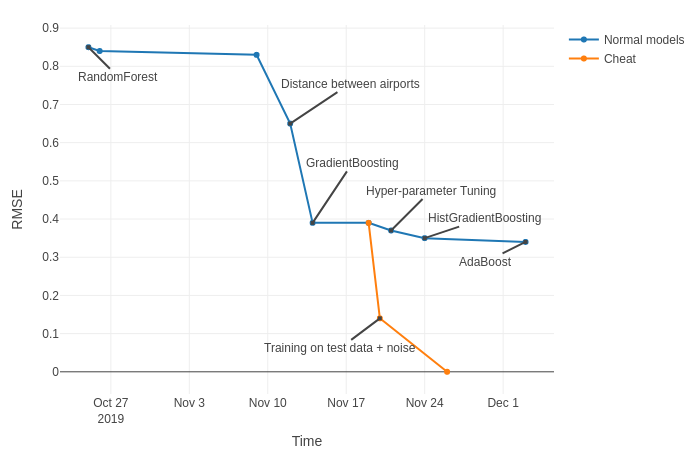
\includegraphics[scale=0.4]{rmse_evolution.png}
\end{figure}

What we can see is that the main changes were due to adding \textbf{new features} to our data, rather than optimizing the hyper-parameters, which often led to overfitting, because of the small amount of data. The methods that were performing best were \textbf{tree based methods}.

\section{Conclusion}

\subsection{Model Interpretability}

\begin{figure}[H]
	\centering
	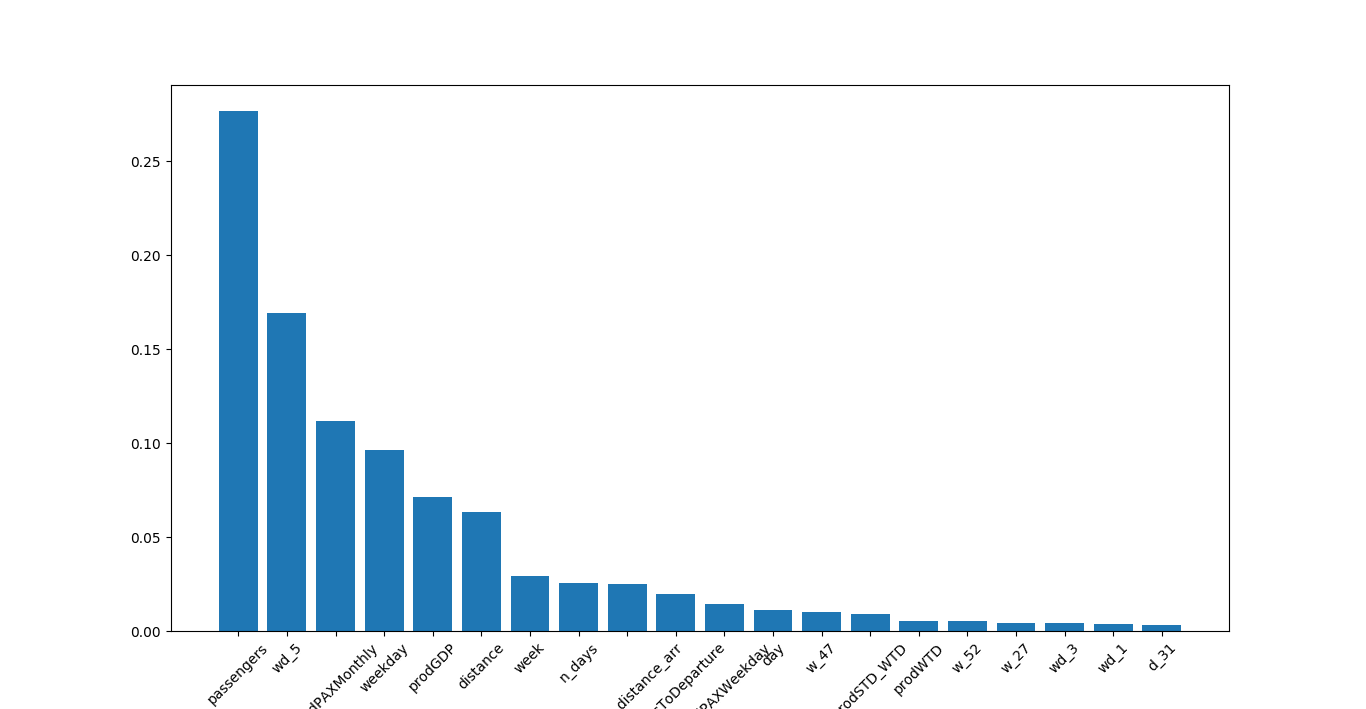
\includegraphics[scale=0.4]{feature_importance.png}
\end{figure}

We can extract several relevant information from the above feature importance graph :

\begin{itemize}
	\item The columns that are an \textbf{interaction} between information of the Departure and the Arrival airports are the ones that are the more relevant. For instance, the \textbf{distance} between airports is our most relevant predictor. This makes sense as the quantity we are trying to estimate is the number of passengers going from a place to another, which also integrates the notion of interaction.
	\item The fact that the date of the flight is a \textbf{Friday} is also a really important feature. This can mean that there are many flights on Friday or that the flight habits of passengers change on Fridays.
\end{itemize}

\subsection{Evaluation of Uncertainty in Predictions}

Because we only have around ten thousand rows of data, we cannot say that our predictions are extremely accurate. It's all the more problematic that the values of log\_PAX are not spread a lot (mostly between 9 and 12). To have a more robust model, we would have needed more data. The lack of data also made it difficult to optimize the hyper-parameters without overfitting.


\subsection{Final Comments and Possible Improvements}

We didn't have time to try the \textit{Time Series} but it would have been interesting to fit a time series on the biggest Departure airports to see how it performed on such data.
Apart from the purely Data Science related improvements we could have done, the infrastructure we have designed could be improved to be made more generic and easier to reuse.

\end{document}
